%
%	Theorieteil
%

\pagebreak
\section{Data Exploration}

\onehalfspacing

\subsection{Location}

Let's start by looking at the number of visitors this year. We can see a huge spike around the global climate strike and Easter.

\begin{figure}[H]
\centering
\caption {Vistors 2021}
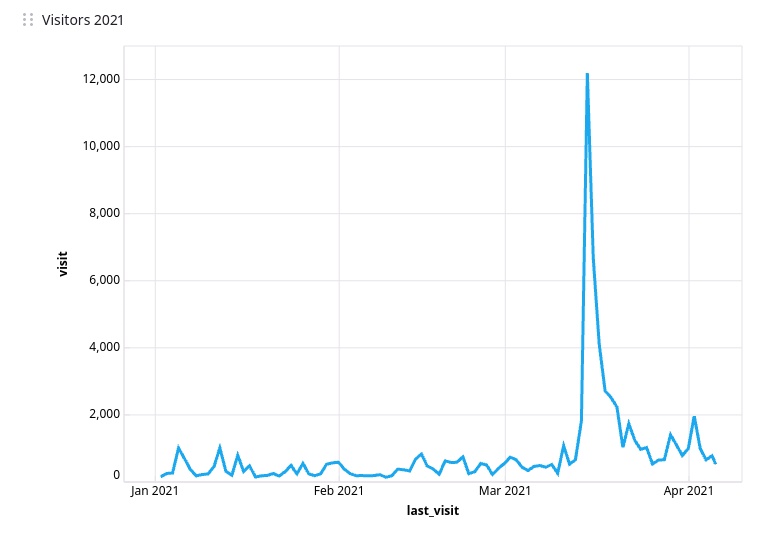
\includegraphics[width=\linewidth]{images/figure01.png}
\label{fig:visitors2021}
\end{figure}

Let's look at the past year. We can see significant spikes around the dates for global and local strikes and local elections.

\begin{figure}[H]
\centering
\caption {Vistors 2020}
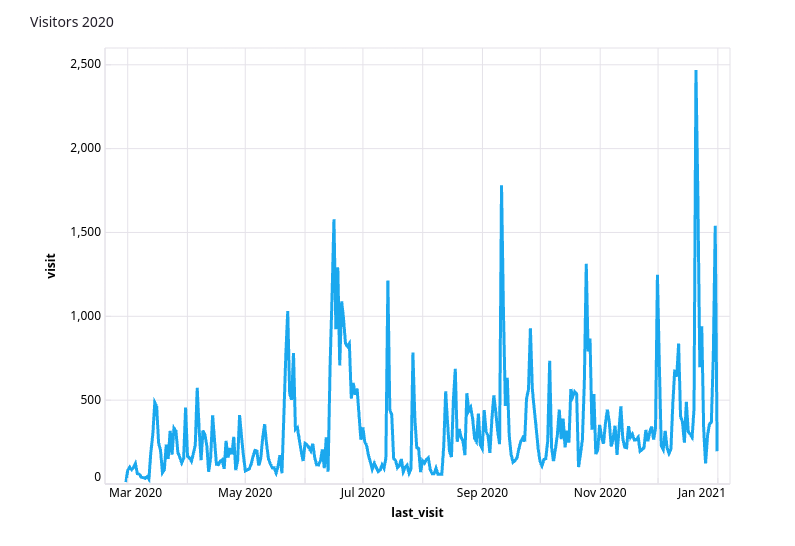
\includegraphics[width=\linewidth]{images/figure02.png}
\label{fig:vistors2020}
\end{figure}

Where do all the users come from?

\begin{figure}[H]
\centering
\caption {Search Engines}
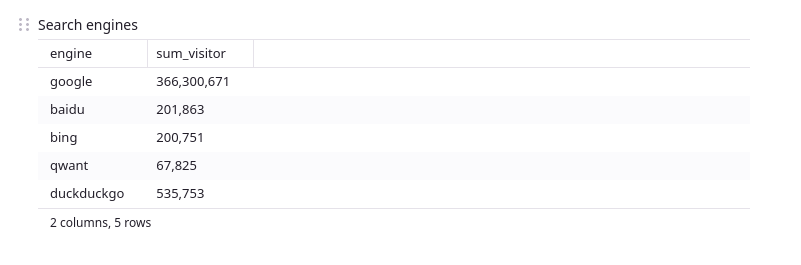
\includegraphics[width=\linewidth]{images/figure03.png}
\label{fig:searchEngines}
\end{figure}

And what are they looking for?

\begin{figure}[H]
\centering
\caption {Search Term Streik}
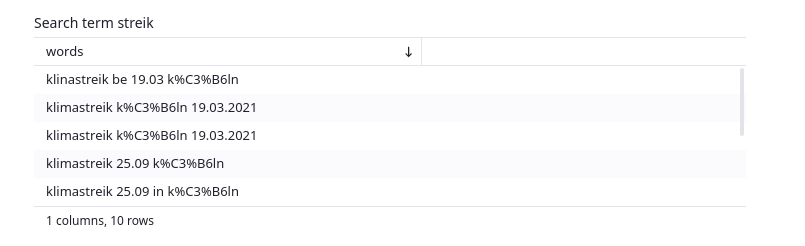
\includegraphics[width=\linewidth]{images/figure04.png}
\label{fig:searchStreik}
\end{figure}

\begin{figure}[H]
\centering
\caption {Search Term Wahl}
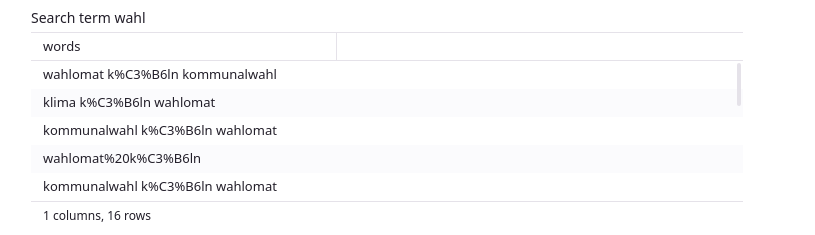
\includegraphics[width=\linewidth]{images/figure05.png}
\label{fig:searchWahl}
\end{figure}

Both the regular climate strikes and the local elections were essential data points, where the community turned to the blog for information.

And where do our admin users come from?

\begin{figure}[H]
\centering
\caption {Admin Access}
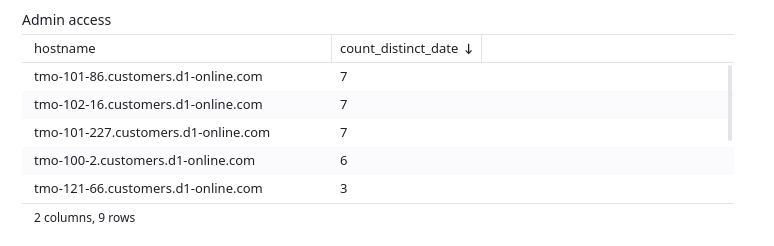
\includegraphics[width=\linewidth]{images/figure06.png}
\label{fig:adminAccess}
\end{figure}

Not surprisingly, with a few exceptions, admin access seems to come from the Deutsche Telekom network, the main carrier in Germany

\subsection{Referrals}

Now, let's look at the referrals:

\begin{figure}[H]
\centering
\caption {Referrals}
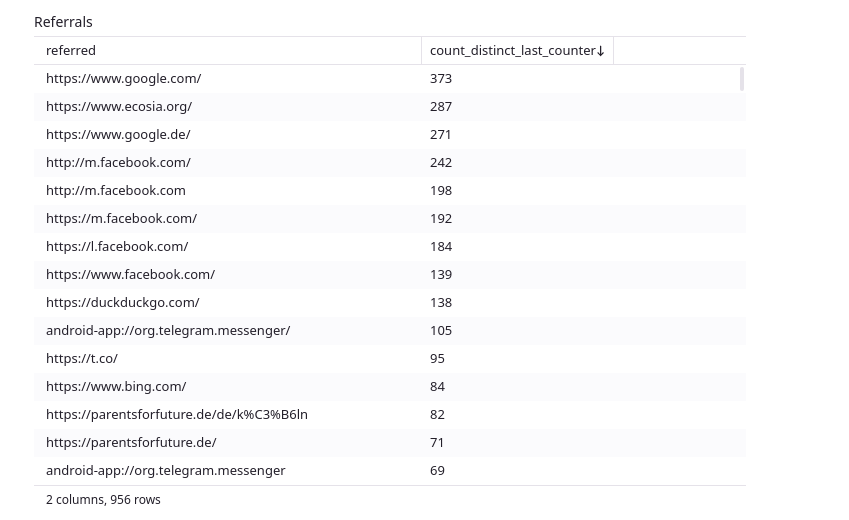
\includegraphics[width=\linewidth]{images/figure07.png}
\label{fig:referrals}
\end{figure}

We see the major search engines in the referrals and the more privacy-oriented ones (\href{https://www.ecosia.org/?c=en}{Ecosia}, \href{https://duckduckgo.com/}{DuckDuckGo}). We can also see several referrals from Twitter and Facebook and the various Telegram channels, indicating a solid connection to the community and integration with other social media sources.

\subsection{Platforms}

As we saw in the referrals, the amount of people using alternative search engines in the climate bubble is quite high. Will we see the same differences when we look at the OS and browser?

\begin{figure}[H]
\centering
\caption {Operating System}
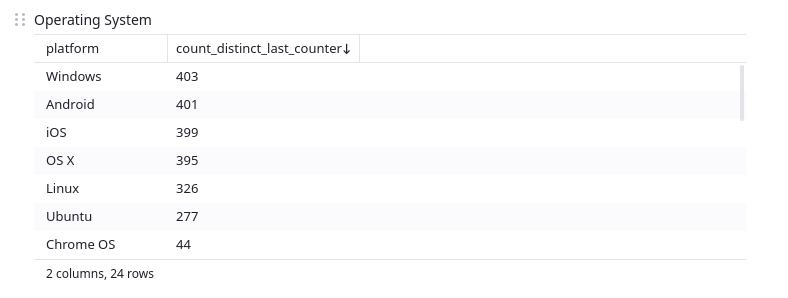
\includegraphics[width=\linewidth]{images/figure08.png}
\label{fig:operatingSystem}
\end{figure}

Access from mobile is pretty evenly split between Android and iOS. Still, the desktop distribution is quite interesting: Even though Windows and Mac OS X are again pretty tight, the number of Linux users is far higher if we add all the distributions. This distribution is very different from the general distribution, where the percentage of Linux users usually is in the lower single digits\footnote{See \textit{Frank, C. (2021)}: Web Traffic Analysis - Predicting Blog Post Performance. \cite{previousBigData}}.

Now, let's look at the browser figures:

\begin{figure}[H]
\centering
\caption {Browser}
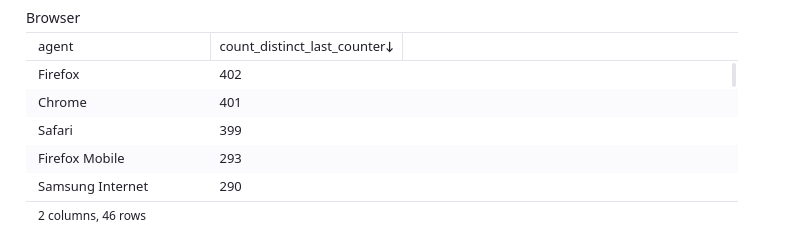
\includegraphics[width=\linewidth]{images/figure09.png}
\label{fig:browser}
\end{figure}

Very different! Firefox and Firefox Mobile together are leading the access, easily outperforming Chrome and Safari. This distribution is a continuation of what we saw before. The climate activist does not like to rely on mainstream search engines, mainstream operating systems, or the mainstream browser.

Firefox, in general, is at approx. 3]\% market share (https://gs.statcounter.com/browser-market-share - see screenshot), even at my blog, it's just at 9\%\footnote{See \textit{Frank, C. (2021)}: Web Traffic Analysis - Predicting Blog Post Performance. \cite{previousBigData}}.

Important lessons to learn:

\begin{itemize}
 \item SEO should focus on Ecosia, DuckDuckGo, and Google
 \item Firefox is the most prevalent browser, and we should optimize the blog theme for it
 \item Linux is the most favored operating system; graphics and images should take that into account
 \item Mobile access is important and should factor in our design
\end{itemize}
